\medskip

On considère une fonction $f$ définie et deux fois dérivable sur $]-2 ~;~+\infty[$. On note $\mathcal{C}_{f}$ sa courbe représentative dans un repère orthogonal du plan, $f'$ sa dérivée et $f''$ sa dérivée seconde.

On a tracé ci-dessous la courbe $\mathcal{C}_{f}$ et sa tangente $T$ au point B d'abscisse $-1$.

On précise que la droite $T$ passe par le point A$(0 ~;~ -1)$.

\begin{center}
		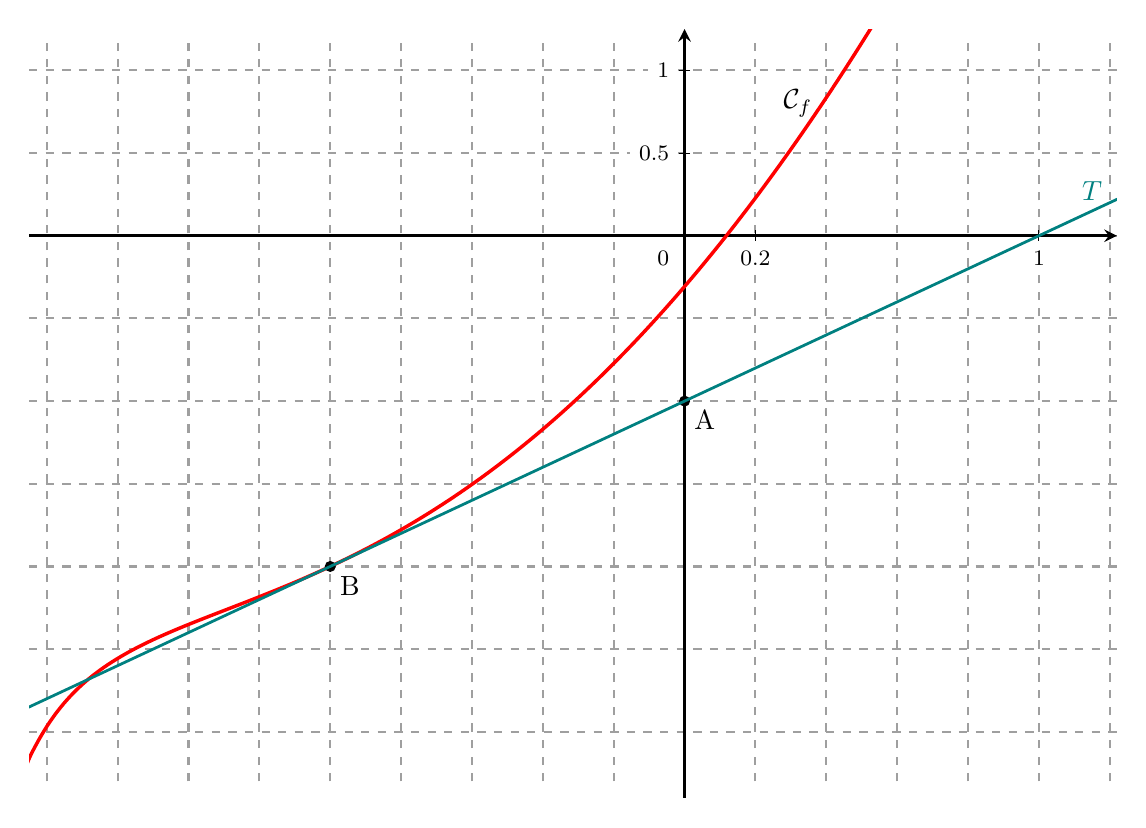
\begin{tikzpicture}[x =45mm,y = 21mm,> = stealth]
			\draw [color = gray!75, line width = 0.75pt, xstep=0.2, ystep = 0.5,dashed] (-1.85,-3.3) grid (1.22,1.2);
			\draw[->,line width=1pt] (-1.85,0) -- (1.22,0);
			\foreach \x in {0.2,1}
			\draw[shift={(\x,0)},color=black] (0pt,2pt) -- (0pt,-2pt) node[below, fill = white] {\footnotesize $\np{\x}$};
			\draw[->,line width=1pt] (0,-3.4) -- (0,1.25);
			\foreach \y in {0.5,1}
			\draw[shift={(0,\y)},color=black] (2pt,0pt) -- (-2pt,0pt) node[left, fill = white] {\footnotesize $\np{\y}$};
			\draw[color=black] (-2pt,-2pt) node[below left] {{\footnotesize  0}};
			\clip (-1.85,-3.4) rectangle (1.22,1.25);
			\draw[line width=1.25pt,color=red,smooth,samples=100,domain= -1.9:0.55 ] plot(\x,{\x*\x+2*\x-1+ln(\x+2)});
			\fill(0,-1) circle (2pt) node[below right]{A};
			\fill(-1,-2) circle (2pt) node[below right]{B};
			\node at (0.32,0.8){\red $ \mathcal{C}_f $};
			\draw[teal,line width=1pt] (-2,-3)--(1.5,0.5)node[pos=0.9,above]{$ T $};
		\end{tikzpicture}
\end{center}

\medskip

\textbf{Partie A : exploitation du graphique.}

\medskip

À l'aide du graphique, répondre aux questions ci-dessous.

\begin{enumerate}
	\item Préciser $f(-1)$ et $f'(-1)$.

	\item La fonction $f$ est-elle convexe sur son ensemble de définition ? Justifier. 

	\item Conjecturer le nombre de solutions de l'équation $f(x) = 0$ et donner une valeur arrondie à $10^{-1}$ près d'une solution.

\end{enumerate}

\medskip

\textbf{Partie B : étude de la fonction }\boldmath $f$ \unboldmath

\medskip

On considère que la fonction $f$ est définie sur $]-2 ~;~+\infty[$ par :

\[f(x) = x^{2}+ 2x - 1 + \ln (x + 2),\]
 où ln désigne la fonction logarithme népérien.

\begin{enumerate}
\item Déterminer par le calcul la limite de la fonction $f$ en $-2$. Interpréter graphiquement ce résultat.

On admet que $\lim\limits_{x  \to +\infty} f(x)=+\infty$.

\item Montrer que pour tout $x>-2, \quad f'(x)=\dfrac{2 x^{2}+6 x+5}{x+2}$.

\item Étudier les variations de la fonction $f$ sur $]-2 ~;~+\infty[$ puis dresser son tableau de variations complet.

\item Montrer que l'équation $f(x)=0$ admet une unique solution $\alpha$ sur $]-2 ~;~+\infty[$ et donner une valeur arrondie de $\alpha$ à $10^{-2}$ près.

\item En déduire le signe de $f(x)$ sur $]-2~;~ +\infty[$.

\item Montrer que $\mathcal{C}_{f}$ admet un unique point d'inflexion et déterminer son abscisse.

\end{enumerate}

\medskip

\textbf{Partie C : une distance minimale.}

\medskip
Soit $g$ la fonction définie sur $]-2 ~;~ +\infty[$ par \quad $g(x)=\ln (x+2)$.

On note $\mathcal{C}_{g}$ sa courbe représentative dans un repère orthonormé $(\mathrm{0} ~;~  \mathrm{I}~,~ \mathrm{J})$, représentée ci-après.

Soit $M$ un point de $\mathcal{C}_{g}$ d'abscisse $x$.

Le but de cette partie est de déterminer pour quelle valeur de $x$ la distance $\mathrm{J}M$ est minimale.

On considère la fonction $h$ définie sur $]-2 ~;~ +\infty[$ par \quad $h(x)=\mathrm{J}M^{2}$.

\begin{center}
		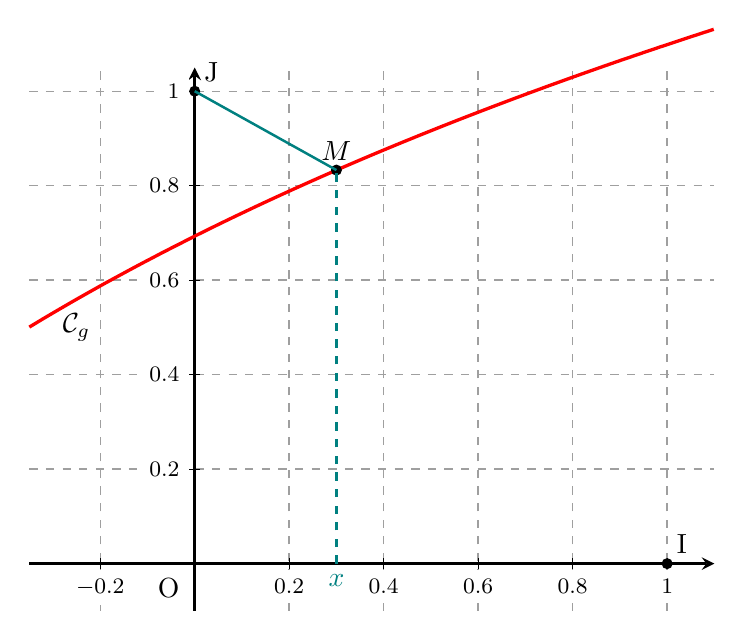
\begin{tikzpicture}[x =60mm,y = 60mm,> = stealth]
			\draw [color = gray!75, line width = 0.5pt, xstep=0.2, ystep = 0.2,dashed] (-0.35,-0.1) grid (1.1,1.05);
			\draw[->,line width=1pt] (-0.35,0) -- (1.1,0);
			\foreach \x in {-0.2,0.2,0.4,0.6,0.8,1}
			\draw[shift={(\x,0)},color=black] (0pt,2pt) -- (0pt,-2pt) node[below, fill = white] {\footnotesize $\np{\x}$};
			\draw[->,line width=1pt] (0,-0.1) -- (0,1.05);
			\foreach \y in {0.2,0.4,0.6,0.8,1}
			\draw[shift={(0,\y)},color=black] (2pt,0pt) -- (-2pt,0pt) node[left, fill = white] {\footnotesize $\np{\y}$};
			\draw[color=black] (-2pt,-2pt) node[below left] {O};
			\draw[line width=1.2pt,color=red,smooth,samples=100,domain= -0.35:1.1 ] plot(\x,{ln(\x+2)});
			\fill(1,0) circle (2pt) node[above right]{I};
			\fill(0,1) circle (2pt) node[above right]{J};
			\fill(0.3,0.833) circle (2pt) node[above]{$ M $};
			\draw[dashed,line width=.9pt, teal] (0.3,0)node[below]{$ x $}--(0.3,0.833);
			\draw[teal,line width=0.9pt](0.3,0.833)--(0,1);
			\node at (-0.25,0.5){$ \mathcal{C}_g $};
		\end{tikzpicture}
\end{center}

\begin{enumerate}
\item Justifier que pour tout $x>-2$, on a : \quad $h(x)=x^{2}+[\ln (x+2)-1]^{2}$.

\item On admet que la fonction $h$ est dérivable sur $]-2 ~;~ +\infty[$ et on note $h'$ sa fonction dérivée.

On admet également que pour tout réel $x>-2$,

$$h'(x)=\dfrac{2 f(x)}{x+2}$$

où $f$ est la fonction étudiée en \textbf{partie B}.

\begin{enumerate}
	\item Dresser le tableau de variations de $h$ sur $]-2 ~;~ +\infty[$.

	\emph{Les limites ne sont pas demandées.}

	\item En déduire que la valeur de $x$ pour laquelle la distance $\mathrm{J}M$ est minimale est $\alpha$ où $\alpha$ est le nombre réel défini à la question \textbf{4.} de la \textbf{partie B}.
\end{enumerate}

\item On notera $M_{\alpha}$ le point de $\mathcal{C}_{g}$ d'abscisse $\alpha$.

	\begin{enumerate}
		\item Montrer que \quad $\ln (\alpha+2)=1-2 \alpha-\alpha^{2}$.

		\item En déduire que la tangente à $\mathcal{C}_{g}$ au point $M_{\alpha}$ et la droite $\left(\mathrm{J}M_{\alpha}\right)$ sont perpendiculaires.

On pourra utiliser le fait que, dans un repère orthonormé, deux droites sont perpendiculaires lorsque le produit de leurs coefficients directeurs est égal à $-1$.
	\end{enumerate}
\end{enumerate}

\bigskip
